\documentclass[twocolumn]{article}
%\documentclass{article}
\usepackage{lipsum}
\usepackage[french]{babel}
\usepackage[T1]{fontenc}
\usepackage[utf8]{inputenc}
\usepackage{hyperref}
\usepackage{setspace}
\usepackage{multicol}
\usepackage{amsfonts}
\usepackage{amsmath}
\usepackage{graphicx}

\doublespacing
\date{}
\author{Redouane ELGHAZI \and Pierre MAHMOUD--LAMY \and Enguerrand PREBET}
\title{Projet de MC2A : Équipe one}

\begin{document}
	\maketitle
	\section{Introduction}
		Le but de ce projet était d'implémenter une méthode de Monte-Carlo par chaînes de Markov appelée algorithme de Metropolis-Hastings. Cet algorithme a pour entrée un ensemble $P$ de points de $\mathbb{R}^N$ et une fonction $\emph{label}^*$ associant un label à chaque point.
		
		Le but de l'algorithme est de trouver une fonction $\emph{label}$ minimisant le nombre de mauvais labels. Dans le cadre de ce projet, la fonction recherchée est de la forme:
		$$\emph{label}(\mathbf{x}) = \text{sign}(\mathbf{w}\cdot \mathbf{x})$$
		Où $w$ est un vecteur de $\big\{{-}1,1\big\}^N$. Cet objectif est modélisé par une énergie proportionnelle au nombre de mauvais labels.
		%Cet objectif est modélisé par l'énergie :		$$E(\mathbf{w}) = \frac{1}{2} \sum_{\mu=1}^{M} (y_\mu - \text{sign}(\mathbf{w}\cdot\mathbf{x}))$$
		
		Pour se faire, à chaque étape, un bit de $\mathbf{w}$ est proposé à la modification, et est accepté avec une probabilité dépendant du nombre de points mal classifiés avant et après modification. La distribution de Boltzmann est utilisée faisant intervenir l'énergie citée précédemment.
	\section{Langage}
		Nous avons choisi d'utiliser deux langages pour ce projet. Un exécutable en C++ exécute le cœur de l'algorithme, ainsi qu'un script en Python pour gérer les appels à cet exécutable ainsi que pour la création de graphes.
		
	\section{Implémentation}
		Le programme en C++ génère $\mathbf{w}^*$ et les $(\mathbf{x}_\mu)$ avant d'effectuer l'algorithme selon les paramètres données en entrée. Selon la question, il écrit dans un fichier les énergies normalisées tout au long de l'algorithme, ou bien uniquement l'énergie normalisée ainsi que le chevauchement entre le modèle original et notre réponse finale.
		
		Comme au plus un bit est changé à chaque itération, il est possible de modifier le label de chaque $\mathbf{x}$ en temps $O(1)$. Cela nous permet d'effectuer une itération en $O(M)$ pour une complexité totale en $O(M(T + N))$ en comptant l'initialisation.
		
	\section{Résultats}
		Nos résultats sont obtenus pour $N=100$, ce qui dans notre implémentation est instantané pour des paramètres adéquats de $\alpha$ et $T$.
		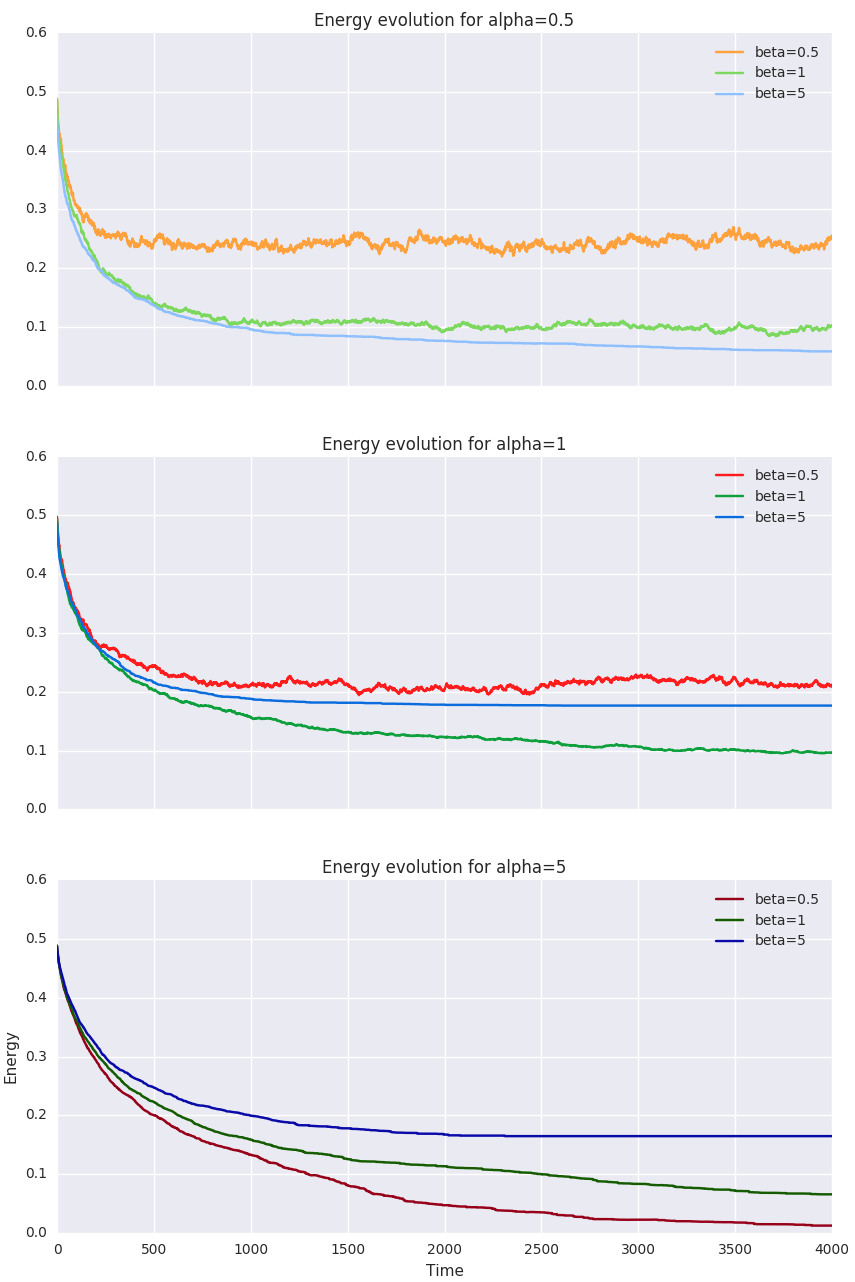
\includegraphics[width=\columnwidth]{../tobekept/ex1_1755923751722050074-r.png}
		On peut remarquer que pour ces 3 tests avec des valeurs $\alpha$ différentes, le $\beta$ optimal diffère, allant du plus grand pour $\alpha = 0.5$, au plus petit pour $\alpha = 5$.
		Cette valeur nous permet aussi d'obtenir une erreur d'au plus 10\% dans les 3 cas.
	\section{Analyse de la valeur de $\beta$}
		oui des plot c'est cool (q2-3)
		puis replot de la q1 avec des beta hinted
	\section{Qu'apporte le simulated annealing}
		encore des plot oui oui des plot
		
		
	\section{Conclusion}
		Je remercie mon manager sans qui rien n'aurait été possible ah non c'est pas les remerciements
\end{document}